\documentclass{CE295_HW_template}

\newcommand{\hmwkNum}{2}
\newcommand{\hmwkTitle}{HW \hmwkNum: State Estimation in Oil Drilling}
\newcommand{\hmwkAuthorName}{Carlin Liao}
\newcommand{\SID}{24358933}

\title{
\vspace{-0.5cm}
\textbf{\hmwkTitle}
\author{} % Leave this blank
\date{} % Leave this blank
\vspace{-1cm}
}

%% Do not edit unless you really know what you are doing.
\documentclass[english]{article}
\usepackage[T1]{fontenc}
\usepackage[latin9]{inputenc}
\usepackage{textcomp}
\usepackage{relsize}

\makeatletter

%%%%%%%%%%%%%%%%%%%%%%%%%%%%%% User specified LaTeX commands.
\def\labnb{0}
\usepackage{hyperref} 
\usepackage{ulem}
\usepackage{latexsym}
\usepackage{amssymb}
\usepackage{amsmath}
\usepackage{amsfonts}
\usepackage{color, colortbl}
\usepackage{graphicx}
\usepackage{lastpage}
\usepackage[framed,numbered,autolinebreaks,useliterate]{mcode}

\newcommand{\red}[1]{{\color{red}#1}}
\newcommand{\blue}[1]{{\color{blue}#1}}
\newcommand{\green}[1]{{\color{green}#1}}

%%%%%%%%%%%%%%%%%%%%%%%%%%%%%%%%%%%%%%%%%%%%%%
\begin{document}
\maketitle
\thispagestyle{fancy}

%---------------
% PROBLEM 1
%---------------

\begin{Problem}[Dynamic System Modeling]

\begin{enumerate}
\renewcommand{\theenumi}{(\alph{enumi})}
    \item We seek to control the bit speed $\omega_B(t)$ using our input $T(t)$ in order to limit oscillations in the drill string.
    
    We have one controllable input $T(t)$ and one uncontrollable input $T_f(t)$.

    Our measured outputs are $\omega_T(t)$ and $\theta_T(t)$ while the performance outputs are $\omega_B(t)$ and $\theta_B(t)$.
    
    Our parameters are $b$, $J_T$, $k$, $b$, and $J_B$.
    
    \item Top: $$J_T \dot{\omega}_T(t) = - k[\theta_T(t) - \theta_B(t)] -b\omega_T(t) + T(t) $$
    Bottom: $$J_B \dot{\omega}_B(t) = k[\theta_T(t) - \theta_B(t)] -b\omega_B(t) - T_f(t) $$
    
    \item State space form is:
    $$
        \begin{bmatrix}
            \omega_T(t) \\
            \omega_B(t) \\
            \dot{\omega}_T(t) \\
            \dot{\omega}_B(t)
        \end{bmatrix} = 
        \begin{bmatrix}
            0 & 0 & 1 & 0 \\
            0 & 0 & 0 & 1 \\
            -\frac{k}{J_T} & \frac{k}{J_T} & -\frac{b}{J_T} & 0 \\
            \frac{k}{J_B} & -\frac{k}{J_B} & 0 & -\frac{b}{J_B}
        \end{bmatrix}
        \begin{bmatrix}
            \theta_T(t) \\
            \theta_B(t) \\
            \omega_T(t) \\
            \omega_B(t)
        \end{bmatrix} +
        \begin{bmatrix}
            0 & 0 \\
            0 & 0 \\
            J_T^{-1} & 0 \\
            0 & -J_B^{-1}
        \end{bmatrix}
        \begin{bmatrix}
            T_T(t) \\
            T_B(t)
        \end{bmatrix}
    $$
    $$
        y(t) = 
        \begin{bmatrix}
            1 & 0 & 1 & 0
        \end{bmatrix}
        \begin{bmatrix}
            \theta_T(t) \\
            \theta_B(t) \\
            \omega_T(t) \\
            \omega_B(t)
        \end{bmatrix}
    $$
    So $$A = \begin{bmatrix}
            0 & 0 & 1 & 0 \\
            0 & 0 & 0 & 1 \\
            -\frac{k}{J_T} & \frac{k}{J_T} & -\frac{b}{J_T} & 0 \\
            \frac{k}{J_B} & -\frac{k}{J_B} & 0 & -\frac{b}{J_B}
        \end{bmatrix} \qquad B = \begin{bmatrix}
            0 & 0 \\
            0 & 0 \\
            J_T^{-1} & 0 \\
            0 & -J_B^{-1}
        \end{bmatrix} \qquad C = \begin{bmatrix}
            1 & 0 & 1 & 0
        \end{bmatrix}$$
    
\end{enumerate}


\end{Problem}

%---------------
% PROBLEM 2
%---------------

\begin{Problem}[Observability Analysis]
$J_T = 100$, $J_B = 25$, $k = 2$, $b = 5$.

\begin{enumerate}
\renewcommand{\theenumi}{(\alph{enumi})}
    \item We see that a column of $\mathcal{O}$ is fully 0 thus the matrix cannot be full rank and the system as-is is not fully observable.
    $$
        \mathcal{O} = 
        \begin{bmatrix}
            1 & 0 & 1 & 0\\
            -\frac{k}{J_T} & \frac{k}{J_T} & 1-\frac{b}{J_T} & 0 \\
            {\frac{k}{J_T}}^2 & {\frac{k}{J_T}}^2 & 1+{\frac{b}{J_T}}^2 & 0 \\
            -{\frac{k}{J_T}}^3 & {\frac{k}{J_T}}^3 & 1-{\frac{b}{J_T}}^3 & 0
        \end{bmatrix}
    $$
    \item Replace $\theta_T - \theta_B$ with $\theta$ (and thus we collapse the first two rows of the state-form with $\omega = \omega_T - \omega_B$
    $$
        \begin{bmatrix}
            \omega(t) \\
            \dot{\omega}_T(t) \\
            \dot{\omega}_B(t)
        \end{bmatrix} = 
        \begin{bmatrix}
            0 & 1 & -1 \\
            -\frac{k}{J_T} & -\frac{b}{J_T} & 0 \\
            \frac{k}{J_B} & 0 & -\frac{b}{J_B}
        \end{bmatrix}
        \begin{bmatrix}
            \theta(t) \\
            \omega_T(t) \\
            \omega_B(t)
        \end{bmatrix} +
        \begin{bmatrix}
            0 & 0 \\
            J_T^{-1} & 0 \\
            0 & -J_B^{-1}
        \end{bmatrix}
        \begin{bmatrix}
            T_T(t) \\
            T_B(t)
        \end{bmatrix}
    $$
    $$
        y(t) = 
        \begin{bmatrix}
            0 & 1 & 0
        \end{bmatrix}
        \begin{bmatrix}
            \theta(t) \\
            \omega_T(t) \\
            \omega_B(t)
        \end{bmatrix}
    $$
    So $$A = \begin{bmatrix}
            0 & 1 & -1 \\
            -\frac{k}{J_T} & -\frac{b}{J_T} & 0 \\
            \frac{k}{J_B} & 0 & -\frac{b}{J_B}
        \end{bmatrix} \qquad B = \begin{bmatrix}
            0 & 0 \\
            J_T^{-1} & 0 \\
            0 & -J_B^{-1}
        \end{bmatrix} \qquad C = \begin{bmatrix}
            0 & 1 & 0
        \end{bmatrix}$$
    \item This new $\mathcal{O}$ still has a column of zeros and is thus also not fully observable.
    $$
        \mathcal{O} = 
        \begin{bmatrix}
            0 & 1 & 0\\
            -\frac{k}{J_T} & -\frac{k}{J_T} & 0 \\
            {\frac{k}{J_T}}^2 & {\frac{k}{J_T}}^2 & 0
        \end{bmatrix}
    $$
\end{enumerate}

\end{Problem}

%---------------
% PROBLEM 3
%---------------

\begin{Problem}[Measurement Data]

\begin{figure}[!htbp]
    \centering
    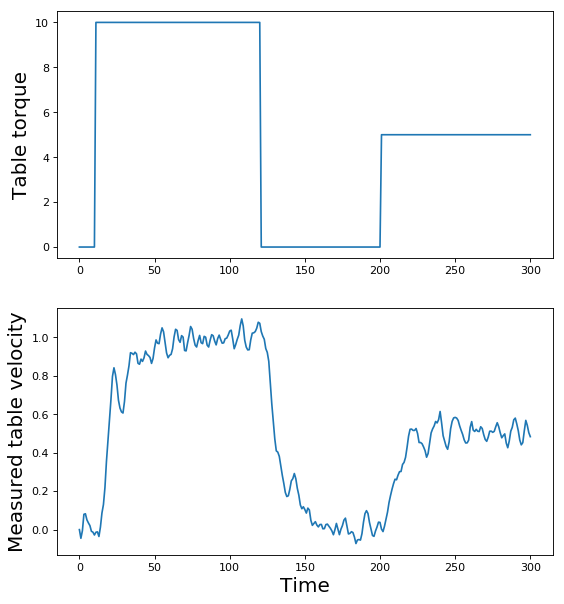
\includegraphics[width=30em]{"imgs/[2] HW2"/q3.png}
    \caption{Torque and velocity over time}
    \label{fig:q3}
\end{figure}


\end{Problem}

%---------------
% PROBLEM 4
%---------------

\begin{Problem}[Luenberger Observer]

\begin{enumerate}
\renewcommand{\theenumi}{(\alph{enumi})}
    \item Eigenvalues:
    $$[-0.08338525+0.29860789j,\quad -0.08338525-0.29860789j,\quad -0.08322949+0.j        ]$$
    Equations:
    $$
        \begin{bmatrix}
            \hat{\omega}(t) \\
            \dot{\hat{\omega}}_T(t) \\
            \dot{\hat{\omega}}_B(t)
        \end{bmatrix} = 
        \begin{bmatrix}
            0 & 1 & -1 \\
            -\frac{k}{J_T} & -\frac{b}{J_T} & 0 \\
            \frac{k}{J_B} & 0 & -\frac{b}{J_B}
        \end{bmatrix}
        \begin{bmatrix}
            \hat{\theta}(t) \\
            \hat{\omega}_T(t) \\
            \hat{\omega}_B(t)
        \end{bmatrix} +
        \begin{bmatrix}
            0 & 0 \\
            J_T^{-1} & 0 \\
            0 & -J_B^{-1}
        \end{bmatrix}
        \begin{bmatrix}
            T_T(t) \\
            T_B(t)
        \end{bmatrix} + 
        L\left(y(t) - \hat{y}(t)\right)
    $$
    $$
    \hat{y}(t) = 
    \begin{bmatrix}
        0 & 1 & 0
    \end{bmatrix} 
    \begin{bmatrix}
        \hat{\theta}(t) \\
        \hat{\omega}_T(t) \\
        \hat{\omega}_B(t)
    \end{bmatrix}
    $$
    \item Per the course notes, as a general rule of thumb we want our $(A-LC)$ eigenvalues to be between two and ten times the size of the largest real part of the eigenvalues of $A$. Thus, I arrived an input eigenvalues of five times the eigenvalues of A, which produces eigenvalues for $(A-LC)$ right in the middle of the rule of thumb range.
    \item $$A_{lobs} = A$$ $$B_{lobs} = \begin{bmatrix} 0 \\ J_T^{-1} \\ 0\end{bmatrix}$$ $$C_{lobs} = C$$
    \item Eigenvalues used as described above. Total RMS error is 0.05536.
        \begin{figure}[!htbp]
            \centering
            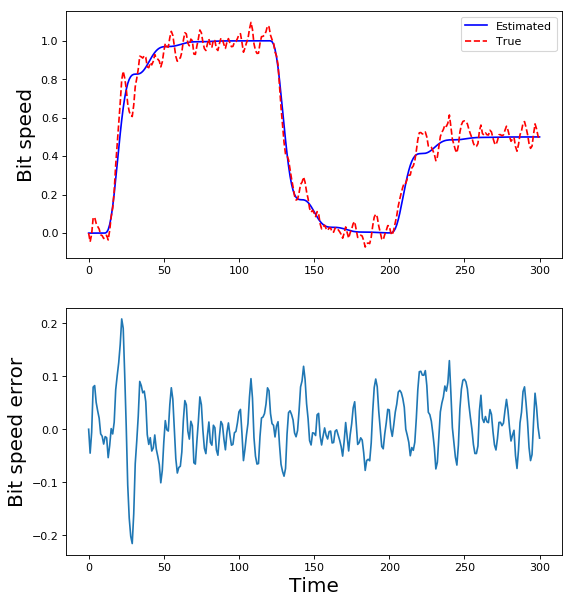
\includegraphics[width=30em]{"imgs/[2] HW2"/q4.png}
            \caption{LO-estimated vs. true velocity over time}
            \label{fig:q4}
        \end{figure}
\end{enumerate}

\end{Problem}

%---------------
% PROBLEM 5
%---------------

\begin{Problem}[Kalman Filter (KF) Design]


\begin{enumerate}
\renewcommand{\theenumi}{(\alph{enumi})}
\item 
$$
    \begin{bmatrix}
        \hat{\omega}(t) \\
        \dot{\hat{\omega}}_T(t) \\
        \dot{\hat{\omega}}_B(t)
    \end{bmatrix} = 
    \begin{bmatrix}
        0 & 1 & -1 \\
        -\frac{k}{J_T} & -\frac{b}{J_T} & 0 \\
        \frac{k}{J_B} & 0 & -\frac{b}{J_B}
    \end{bmatrix}
    \begin{bmatrix}
        \hat{\theta}(t) \\
        \hat{\omega}_T(t) \\
        \hat{\omega}_B(t)
    \end{bmatrix} +
    \begin{bmatrix} 0 \\ J_T^{-1} \\ 0\end{bmatrix}
    \begin{bmatrix}
        T_T(t)
    \end{bmatrix} + 
    L(t)\left(y_m(t) - \hat{y}(t)\right)
$$
$$
    \hat{y}(t) = 
    \begin{bmatrix}
        0 & 1 & 0
    \end{bmatrix} 
    \begin{bmatrix}
        \hat{\theta}(t) \\
        \hat{\omega}_T(t) \\
        \hat{\omega}_B(t)
    \end{bmatrix}
$$
$$
    L(t) = \Sigma(t) C^T N^{-1},\qquad \forall t>0
$$
$$
    \dot{\Sigma}(t) = \Sigma(t) A^T + A \Sigma(t) + W - \Sigma(t) C^T N^{-1} C \Sigma(t),\qquad \Sigma(0) = \Sigma_0
$$
\item Without a rule of thumb like with the Luenberger observer, I tried different combinations for the three entries of $W$ (as we assume a diagonal, uncorrelated multivariate distribution). It took me a few tries to beat my initial guess of $[0.1, 0.01, 0.1]$ inspired by the orders of magnitude in the course notes example, and I danced around with different orders before arriving at $[1, 0.01, 0.1]$.

\item Kalman Filter RMSE: 0.0469337462244 rad/s
    \begin{figure}[!htbp]
        \centering
        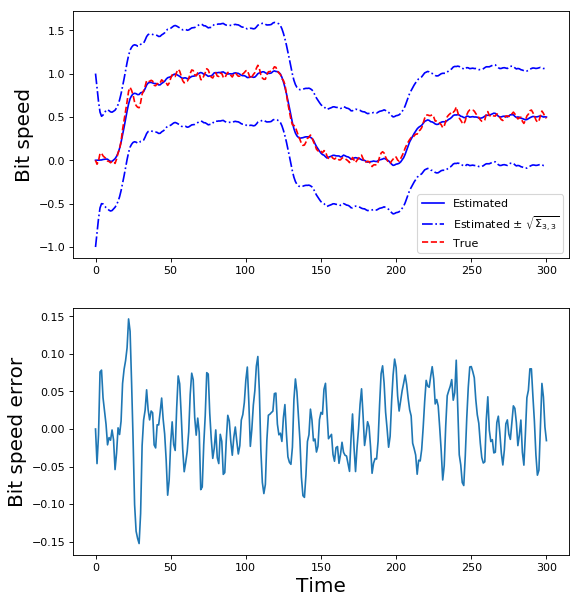
\includegraphics[width=30em]{"imgs/[2] HW2"/q5.png}
        \caption{KF-estimated vs. true velocity over time}
        \label{fig:q5}
    \end{figure}

\item We have $eig(A-L(300)C)$ values of 
$$[-0.18107734+0.28976716j, -0.18107734-0.28976716j, -0.66697227+0.j]$$
which have the same sign (as required) and the same order of magnitude as my poles for the Luenberger observer
$$[-0.41692625+1.49303945j -0.41692625-1.49303945j -0.41614745+0.j  ]$$
 but are otherwise are dissimilar.

\end{enumerate}



\end{Problem}

%---------------
% PROBLEM 6
%---------------

\begin{Problem}[Extended Kalman Filter (EKF) Design]

$$J_T \dot{\omega}_T(t) = - (k_1\theta(t) + k_2 \theta^3(t)) -b\omega_T(t) + T(t) $$
$$J_B \dot{\omega}_B(t) = (k_1\theta(t) + k_2 \theta^3(t)) -b\omega_B(t) - T_f(t) $$

$$
\begin{bmatrix}
    \hat{\omega}(t) \\
    \dot{\hat{\omega}}_T(t) \\
    \dot{\hat{\omega}}_B(t)
\end{bmatrix} = 
\begin{bmatrix}
    0 & 1 & -1 \\
    -\frac{k_1}{J_T} & -\frac{b}{J_T} & 0 \\
    \frac{k_1}{J_B} & 0 & -\frac{b}{J_B}
\end{bmatrix}
\begin{bmatrix}
    \hat{\theta}(t) \\
    \hat{\omega}_T(t) \\
    \hat{\omega}_B(t)
\end{bmatrix} +
\begin{bmatrix}
    0 & 0 & 0 \\
    -\frac{k_2}{J_T} & 0 & 0 \\
    \frac{k_2}{J_B} & 0 & 0
\end{bmatrix}
\begin{bmatrix}
    \hat{\theta}(t) \\
    \hat{\omega}_T(t) \\
    \hat{\omega}_B(t)
\end{bmatrix}^3 +
\begin{bmatrix} 0 \\ J_T^{-1} \\ 0\end{bmatrix}
\begin{bmatrix}
    T_T(t)
\end{bmatrix} + 
L(t)\left(y_m(t) - 
    \begin{bmatrix}
        0 & 1 & 0
    \end{bmatrix} 
    \begin{bmatrix}
        \hat{\theta}(t) \\
        \hat{\omega}_T(t) \\
        \hat{\omega}_B(t)
    \end{bmatrix}
\right)
$$
\begin{align*}
F(t) &= \frac{\partial}{\partial x} \left( 
    \begin{bmatrix}
        0 & 1 & -1 \\
        -\frac{k_1}{J_T} & -\frac{b}{J_T} & 0 \\
        \frac{k_1}{J_B} & 0 & -\frac{b}{J_B}
    \end{bmatrix}
    \begin{bmatrix}
        \hat{\theta}(t) \\
        \hat{\omega}_T(t) \\
        \hat{\omega}_B(t)
    \end{bmatrix} +
    \begin{bmatrix}
        0 & 0 & 0 \\
        -\frac{k_2}{J_T} & 0 & 0 \\
        \frac{k_2}{J_B} & 0 & 0
    \end{bmatrix}
    \begin{bmatrix}
        \hat{\theta}(t) \\
        \hat{\omega}_T(t) \\
        \hat{\omega}_B(t)
    \end{bmatrix}^3
\right) \\
&= \begin{bmatrix}
        0 & 1 & -1 \\
        -\frac{k_1}{J_T} & -\frac{b}{J_T} & 0 \\
        \frac{k_1}{J_B} & 0 & -\frac{b}{J_B}
    \end{bmatrix} + 
    \begin{bmatrix}
        0 & 0 & 0 \\
        -3\frac{k_2}{J_T} & 0 & 0 \\
        3\frac{k_2}{J_B} & 0 & 0
    \end{bmatrix}
    \begin{bmatrix}
        \hat{\theta}(t) \\
        \hat{\omega}_T(t) \\
        \hat{\omega}_B(t)
    \end{bmatrix}^2 \\
H(t) &= \frac{\partial}{\partial x} \left( 
    \begin{bmatrix}
        0 & 1 & 0
    \end{bmatrix} 
    \begin{bmatrix}
        \hat{\theta}(t) \\
        \hat{\omega}_T(t) \\
        \hat{\omega}_B(t)
    \end{bmatrix}
\right) \\
&= C\\
L(t) &= \Sigma(t) H^T N^{-1},\qquad \forall t>0\\
\dot{\Sigma}(t) &= \Sigma(t) F(t)^T + F(t) \Sigma(t) + W - \Sigma(t) H(t)^T N^{-1} H(t) \Sigma(t),\qquad \Sigma(0) = \Sigma_0
\end{align*} 

Extended Kalman Filter RMSE: 0.0450165889712 rad/s
    \begin{figure}[!htbp]
        \centering
        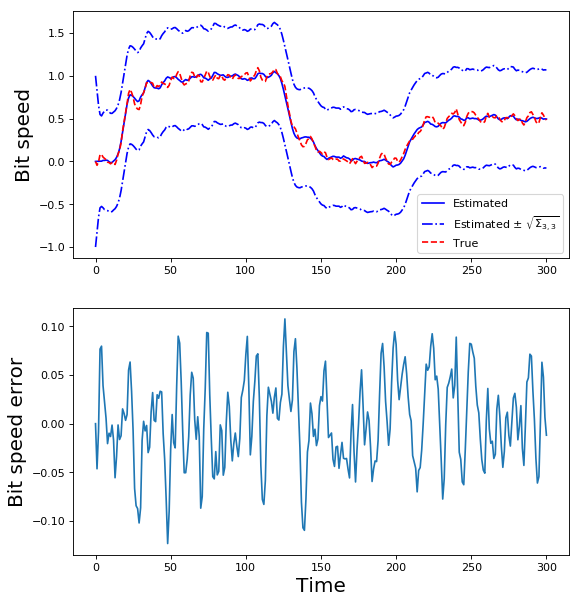
\includegraphics[width=30em]{"imgs/[2] HW2"/q6.png}
        \caption{EKF-estimated vs. true velocity over time}
        \label{fig:q6}
    \end{figure}



\end{Problem}

\end{document}
